\chapter{Introducción}

Desde mediados de siglo XX, la popularización de la radio posibilitó la aparición de un nuevo tipo de medio de comunicación, que recibieron varias denominaciones: ``libres'', ``comunitarias'', ``piratas'', ``locales''. A pesar de la diversidad de nombres, todas compartían un mismo objetivo global: brindar voz a los que normalmente no acceden a los medios masivos y comerciales, democratizar la palabra.\\

En Latinoamérica, aunque la primer radio de estas características comenzó a emitir desde 1947 (radio Sucre, Bolivia), no sería hasta la finalización de las dictaduras militares (años 80') que el fenómeno explotara, con el surgimiento de emisoras comunitarias a lo largo y ancho del continente.\footnote{Rubén Petrucci, ``Características de la radio comunitaria'', \href{http://proarpi.blogspot.com/2006/12/caracteristicas-de-la-radio-comunitaria.html}{proarpi.blogspot.com/2006/12/caracteristicas-de-la-radio-comunitaria.html}}
\\

Uruguay no es una excepción a esto, y desde el año 1986 se registran diversas experiencias de radios comunitarias. Debido a su ilegalidad y persecución, a su estigmatización de ``piratas'', las trayectorias de las mismas fueron accidentadas, y en muchos casos el resultado final fue el silencio en el dial... Para fortalecerse, las radios crearon organizaciones que las nuclean, siendo AMARC-Uruguay (Asociación Mundial de Radios Comunitarias) y ECOS (Coordinadora de Radios Comunitarias del Uruguay) los principales referentes en la actualidad. A partir de 2007, la situación legal de las radios comunitarias cambió radicalmente, con la aprobación de la ley 18.232 ``Servicio de Radiodifusión Comunitaria''.\\

La Asociación Mundial de Radios Comunitarias (AMARC) es el referente organizacional, político y comunicacional de un movimiento internacional constituido en torno a las radios comunitarias, ciudadanas y alternativas. Reconocida como organismo no gubernamental, respresenta a radios comunitarias de todas partes del mundo, buscando promover la democratizacion de la palabra. Es una organización sin fines de lucro, de carácter laico, cuya misión es promover la democratización de las comunicaciones para favorecer la libertad de expresión y contribuir al desarrollo equitativo de la sociedad. En nuestro país, AMARC-Uruguay se encuentra trabajando en la línea estratégica de buscar el fortalecimiento de las radios comunitarias desde hace 15 años. Sin desconocer este proceso, este proyecto se propuso acompañar a través de dos objetivos concretos esta línea de trabajo.\\

Ahora bien, ¿qué es una radio comunitaria?. Existen hoy día en la región diferentes definiciones: “comunitarias”, “alternativas”, “ciudadanas”, “populares”. En el caso de Uruguay, las mismas emisoras han optado por el término comunitarias.\\

Para definir una radio comunitaria, se hará uso de la propia definición que AMARC-Uruguay hace de sí misma en su declaración de Principios, votados y aprobados en su Asamblea del 9 de diciembre de 2007. Se autodefinen como actores privados de propiedad colectiva, con una finalidad pública. Tienen por definición una finalidad social y una programación altamente participativa. Su misión es colaborar con la democratización de la sociedad, desde la democratización de la palabra. Son emprendimientos sociales no lucrativos, que responden a principios de independencia y pluralidad. Entienden que se diferencian de otras emisoras por su rentabilidad sociocultural, por su búsqueda expresa de construir ciudadanía, así como por su intención de representar los intereses de su comunidad, sea ésta una pequeña localidad o un amplio sector social. Lo comunitario no hace referencia precisamente a un lugar pequeño, sino a un espacio de intereses compartidos. Los medios comunitarios defienden la diversidad de idiomas y culturas, los Derechos Humanos en un sentido amplio y la equidad de género. Por último, está en sus principios básicos la solidaridad entre las diferentes emisoras asociadas.\footnote{Extraído de: \href{http://amarcuruguay.org/content/view/88/52}{amarcuruguay.org/content/view/88/52}}\\

En diciembre de 2007, se aprobó la Ley de servicio de Radiodifusión Comunitaria. El nuevo marco legal permite regular la situación de las mismas, y garantizar sus derechos, pero también es generadora de obligaciones, implicando un nuevo desafío.\\

Entonces, la radio comunitaria constituye un espacio para el ejercicio de la ciudadanía, en tanto forma de organización ciudadana, autogestionaria y autónoma, donde se expresan intereses colectivos, político-culturales en el marco de un proyecto comunicacional. A través de estas organizaciones, las personas pueden hacer uso de sus derechos a la comunicación y a la expresión. La comunidad puede tener voz, colectivizar sus necesidades, conflictos, inquietudes, y dialogar también en fin de buscar soluciones, de construir desde lo colectivo.
\newpage
\section{Construcción de la demanda y formulación del proyecto}

Este proyecto nace en el marco de un vínculo entre actores de radios comunitarias y algunos de los integrantes del equipo universitario. La construcción de la demanda, tiene como punto de partida la asistencia a un taller nacional de AMARC realizado en mayo de 2009, en el cual  el colectivo de radios analizó críticamente algunos aspectos de la sustentabilidad, los que sirvieron como base para la formulación del proyecto.\\

El primer objetivo específico consistía en realizar una sistematización y colectivización de saberes de las radios en lo relativo a su gestión.\\

La gestión de las radios implica varias dimensiones que debieron ser trabajadas con cada colectivo:\\

\begin{itemize}
  \item Comunicación interna
  \item Comunicación con la comunidad
  \item Comunicación con la red de AMARC
  \item Recursos financieros
  \item Técnicos
  \item Organización interna
  \item Fuentes de información
\end{itemize}

Asimismo, se pretendía trabajar con cada colectivo en torno a la historia de cada radio y su agenda en 2010, de modo de poder confeccionar una historia de la red.\\

En intercambio con la mesa de AMARC, se planteó otro objetivo específico: el estudio de audiencia, tarea que la organización tiene pendiente desde sus comienzos y no ha podido ejecutar por falta de recursos. Consiste en caracterizar la población en cuanto a sus preferencias, así como estudiar su conocimiento y opinión en cuanto a las radios comunitarias.\\

Las etapas del proyecto eran:

\begin{enumerate}
  \item Relevamiento: trabajo con el colectivo de cada radio, en torno a los objetivos específicos.
  \item Sistematización: generación de documentos que sinteticen los puntos del relevamiento de saberes y procesamiento de la encuesta.
  \item Taller nacional: presentación de la sistematización a los representantes de todos los colectivos, con el fin de realizar modificaciones y agregados.
  \item Sistematización final: tomando como insumo lo trabajado en el taller nacional, preparar una publicación que dé cuenta de los resultados del proyecto.
\end{enumerate}


El proyecto fue aprobado en setiembre de 2009 por la Comisión Sectorial de Extensión y Actividades en el Medio (CSEAM) de la Universidad de la República, en el marco del llamado a proyectos estudiantiles de extensión\footnote{Los llamados a proyectos de extensión son gestionados por la Unidad de Proyectos del Servicio Central de Extensión: \href{http://www.extension.edu.uy/proyectos}{www.extension.edu.uy/proyectos}.}, obteniéndose un financiamiento de $\$$40.000 (alrededor de 2.000 USD) para ejecutarse en un año. En los siguientes meses de ese año se diseñaron específicamente las estrategias para lograr los objetivos específicos. Se elaboraron dos documentos de base, definiendo la metodología del estudio de audiencia y del relevamiento de saberes. Se determinó un número mínimo de 769 encuestas para tener un error menor al $5\%$ en el estudio de audiencia. La encuesta fue diseñada tomando como antecedente una realizada en El Puente FM en 2002, por los licenciados Díaz y Pagés. Cuenta con cuatro partes:\\

\begin{enumerate}
  \item Información general
  \item Hábitos de radioescucha
  \item Radios comunitarias en general
  \item Radio comunitaria afiliada a AMARC de la zona encuestada
\end{enumerate}


La definición del formato final de la encuesta se realizó en conjunto con la mesa nacional de AMARC. Para probar su funcionamiento en campo se realizó un ensayo piloto, en la zona del Cerro, con alrededor de 20 encuestas, donde se efectuaron algunos ajustes.\\

\section{El recorrido}

El trabajo de campo se realizó en varias etapas, teniendo una duración aproximada de 6 meses.\\

Desde una perspectiva que considera la descentralización, se partió de los puntos más lejanos a la capital. En estos casos se realizaron dos viajes, por una parte la zona del litoral, y por otra la zona este, donde se visitaron varias radios en dos fines de semana de febrero y abril respectivamente. Las visitas a las radios de los departamentos de Montevideo, San José y Canelones se realizaron en una última etapa, desde mayo hasta agosto. A continuación, se describe lo realizado radio a radio, en orden cronológico.\\
\begin{figure}[htpb]
 \centering
 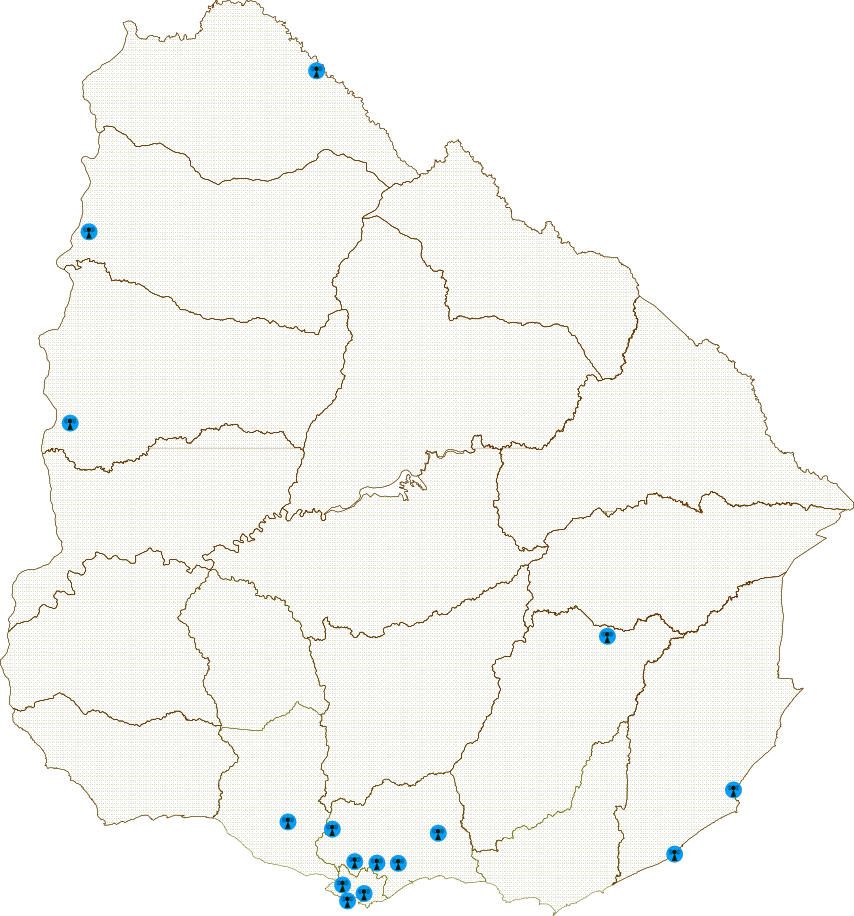
\includegraphics[scale=0.6]{./Cap/imestaud/MapaTotal.png}
 % MapaTotal.png: 854x916 pixel, 120dpi, 18.08x19.39 cm, bb=0 0 512 550
 \caption{Mapa de las radios comunitarias asociadas a AMARC que participaron en el proyecto de extensión universitaria Las Radios no son Ruido.}
 \label{MapaTotal}
\end{figure}

\subsection{Zona Norte}
\begin{figure}[htbp!]
 \centering
 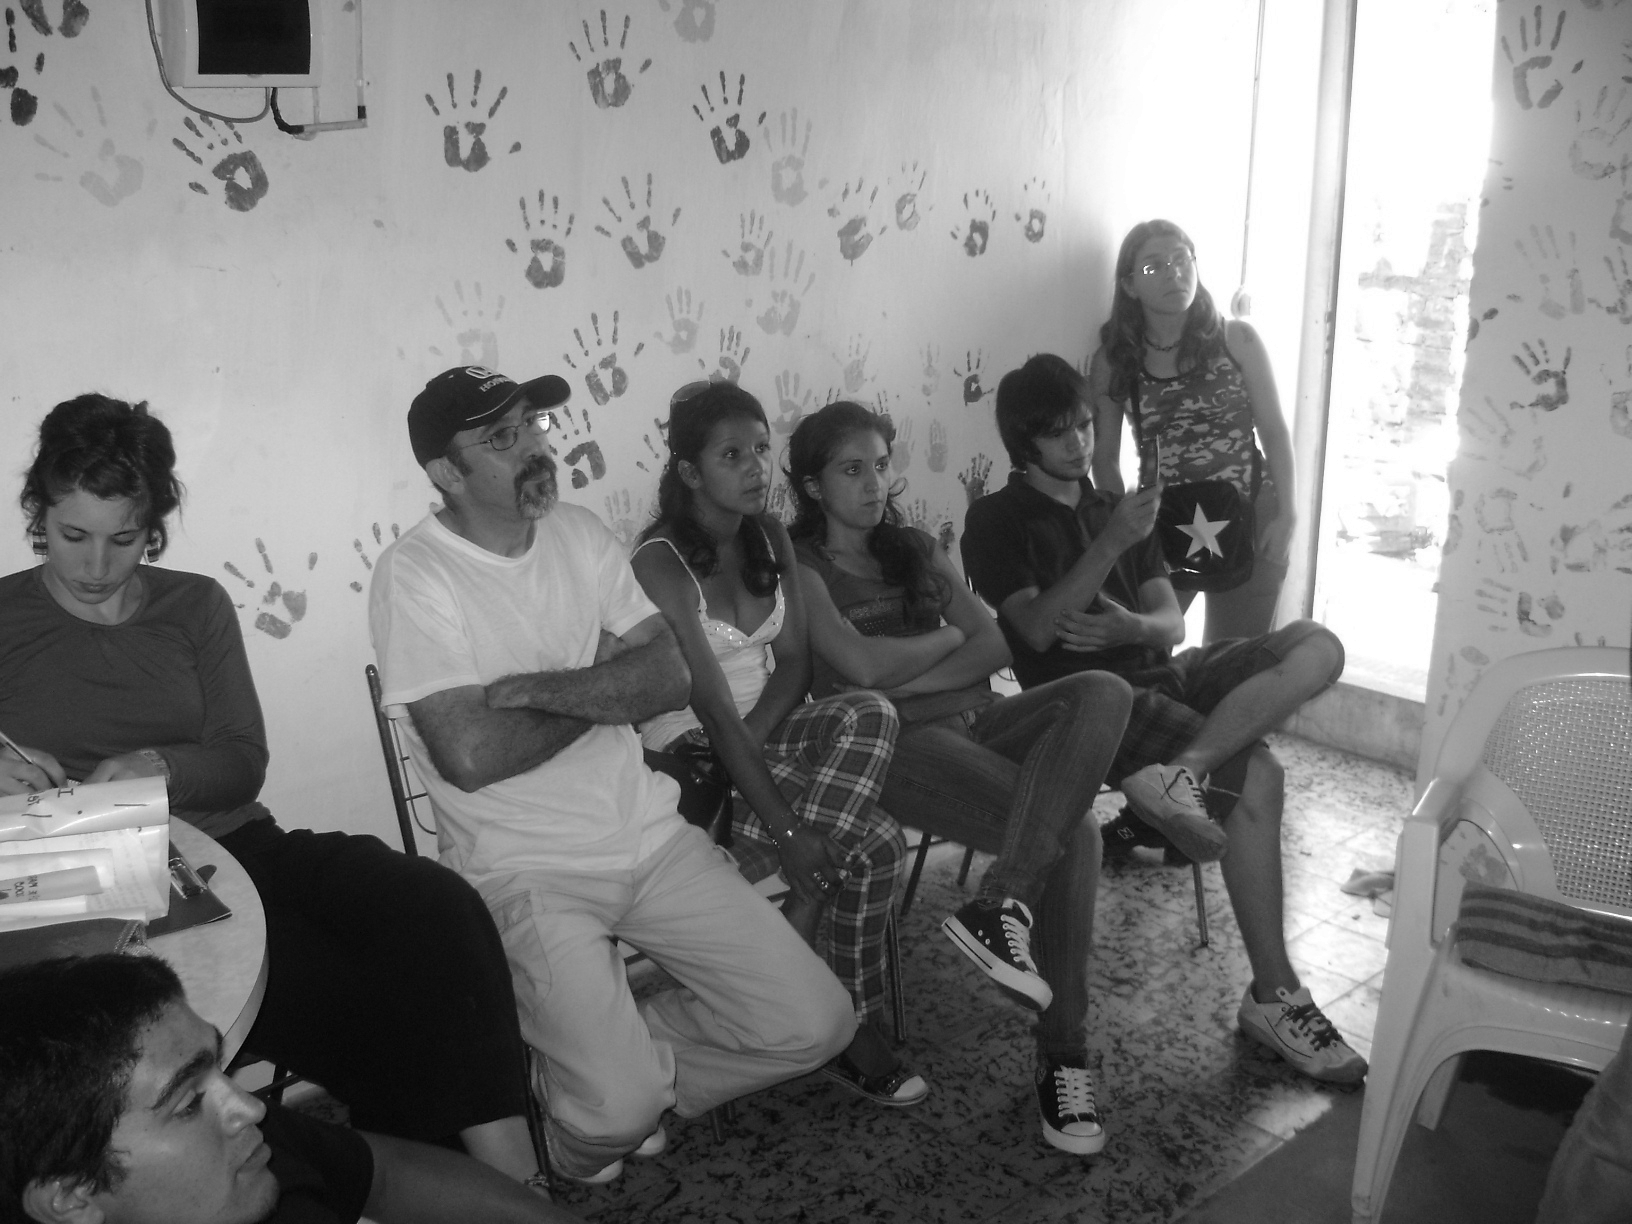
\includegraphics[scale=0.15,keepaspectratio=true]{./Cap/Fotos/HorizontePay.jpg}
 % HorizontePay.jpg: 1632x1224 pixel, 72dpi, 57.57x43.18 cm, bb=
 \caption{Taller en radio Horizonte, Paysandú.}
 \label{HorizontePay}
\end{figure}

\textbf{“Horizonte Max”. Artigas.} Se realizó el taller en un salón comunal, con gran parte del colectivo. En el mismo, los participantes hacen hincapié en la gran saturación de radios de tipo comunitario (aunque no comprendidas dentro del censo de URSEC), la problemática de relacionamiento con dichas radios, además de la recepción de radios brasileras, las cuales interfieren en la correcta recepción de señales propias del departamento.\\

\textbf{“Impactos”. Salto.} El lugar de trabajo fue el club social y deportivo La Paloma, donde se encuentran las instalaciones de la radio. El taller no se pudo instrumentar por la escasa asistencia del colectivo, realizando de modo parcial las tareas propuestas.\\

\textbf{“Horizonte”. Paysandú.} Se realizó el taller en la propia radio con gran participación de los miembros de la misma. Se trataba de un colectivo joven con gran receptividad a la propuesta.\\

\subsection{Zona Este}

\textbf{“Radio Parque”. La Paloma, Rocha.} El encuentro se realizó en las instalaciones de la vieja estación de AFE con dos integrantes de la radio, que actualmente sostienen el proyecto radial. Igualmente se pudo instrumentar el taller y posteriormente se realizaron las encuestas.\\

\textbf{“El Capiz”. Valizas, Rocha.} El taller se realizó en las instalaciones de la radio con la mayoría del colectivo, no así las encuestas, las cuales quedaron en manos de los integrantes de la radio para su posterior realización por iniciativa propia.\\

\textbf{“La Heladera”. José Pedro Varela, Lavalleja.} El taller se realizó en el local de la radio con gran participación del colectivo. En la realización de las encuestas colaboraron la mayoría de sus miembros.\\

\subsection{Montevideo, San José y Canelones}
\begin{figure}[htbp!]
 \centering
 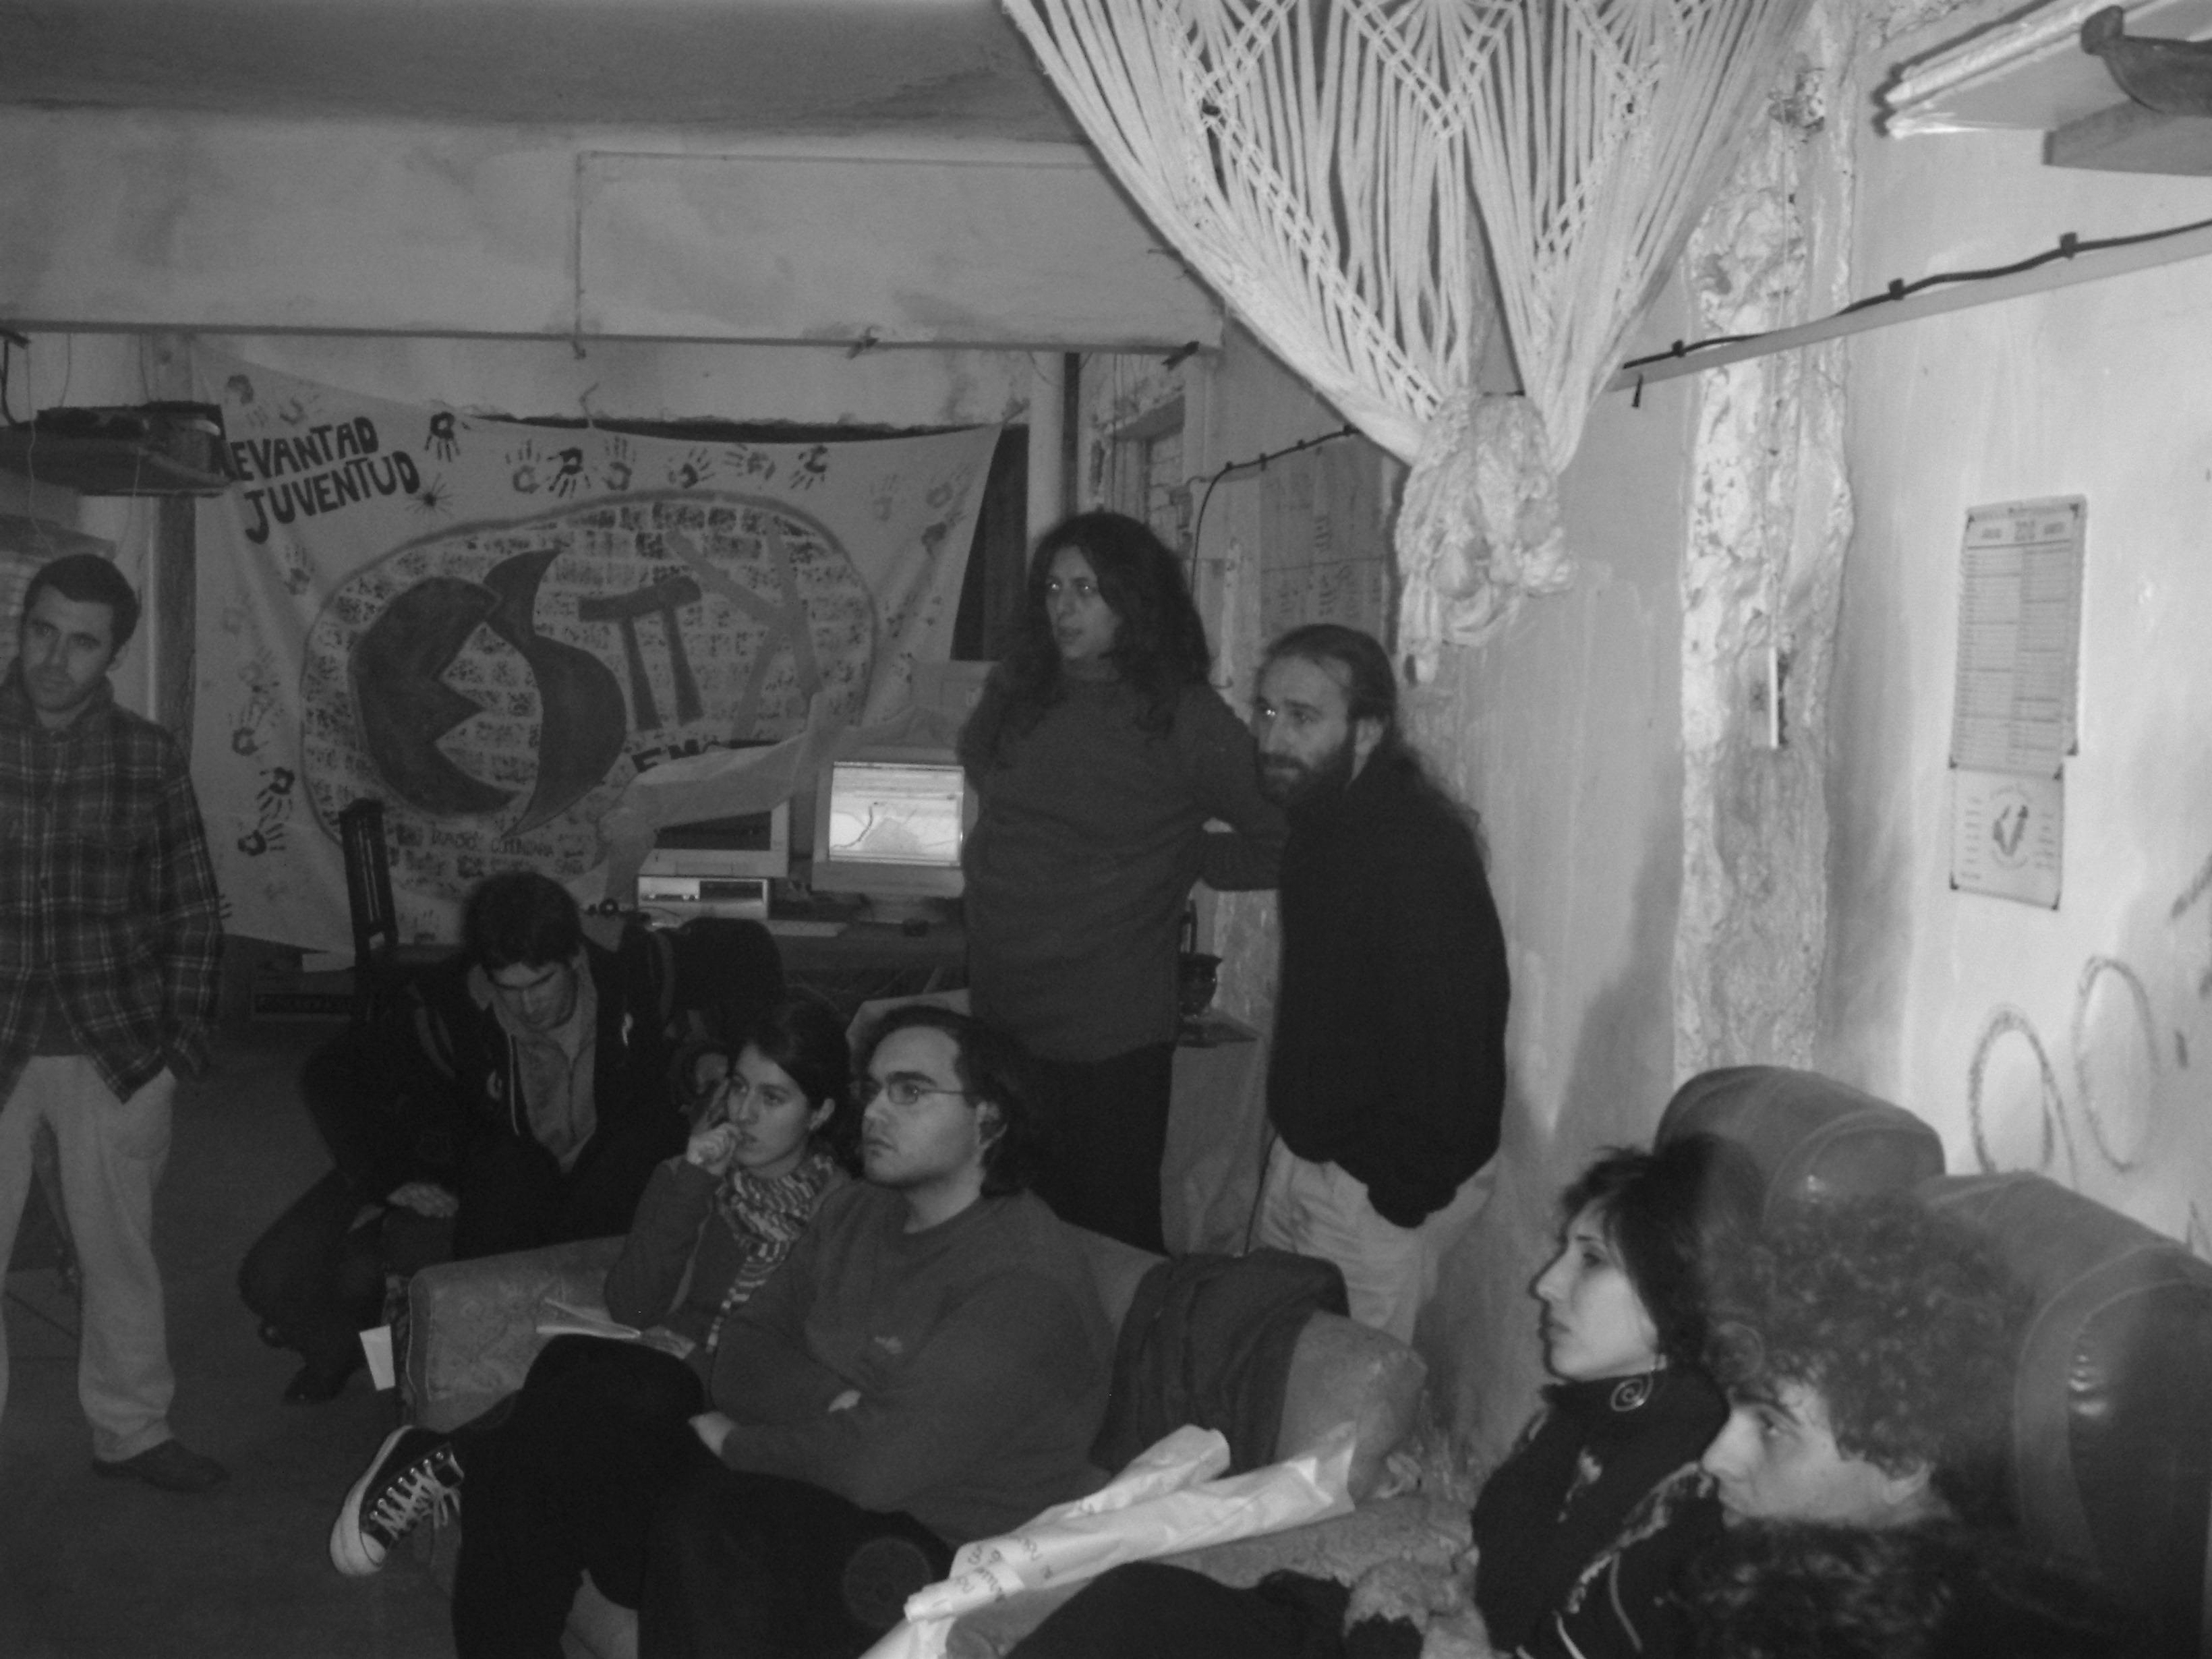
\includegraphics[scale=0.1,keepaspectratio=true]{./Cap/Fotos/Espikabyn.jpg}
 % Espikabyn.jpg: 3280x2460 pixel, 96dpi, 86.78x65.09 cm, bb=
 \caption{Taller en radio Espika, Santa Lucía, Canelones.}
 \label{Espika}
\end{figure}
\textbf{“Universo”. Montes, Canelones.} Se caracteriza por tener un colectivo numeroso y por ser la única señal de radio local. El taller se realizó con la mayoría de sus integrantes y las encuestas no tuvieron participación por parte de los miembros de la radio.\\

\textbf{“Radio Prado”. Paso de la Arena, Montevideo.} Se realizó una reunión previa al trabajo propuesto, dado que el colectivo había pasado por varios encuentros con otros proyectos universitarios con los cuales no habían tenido buenas experiencias. El encuentro se realizó en las instalaciones de la radio, ubicada en la casa de uno de los integrantes. Dicha reunión se caracterizó por una buena participación del colectivo de la radio, contando incluso con una integrante que se encontraba en Estados Unidos, que participó mediante teleconferencia.\\

\textbf{“Vilardevoz”. Reducto, Montevideo.} La primer actividad realizada fueron las encuestas con participación de integrantes de la radio. El taller se realizó dentro de las instalaciones de la radio las cuales se encuentran en el propio hospital. Colectivo numeroso compuesto por usuarios del hospital y el equipo técnico.\\

\textbf{“General Artigas”. Toledo, Canelones.} Se trabajó con un colectivo numeroso, el cual poseía una grilla muy variada en programación. La encuesta fue realizada por los integrantes de la radio en otra ocasión.\\

\textbf{“Espika”. Santa Lucía, Canelones.} El taller se realizó en las instalaciones de la radio, un local alquilado cerca del centro de la ciudad. El colectivo era pequeño, y participó en toda la actividad. La radio está inmersa en un proyecto multicultural el cual forma parte de distintas actividades artísticas y culturales. En la realización de las encuestas participaron integrantes de la radio.\\

\textbf{“Timbó”. San José.} El taller se realizó con la mayoría del colectivo y posteriormente se realizaron las encuestas en conjunto con integrantes de la radio. El grupo era pequeño y contaba con local propio, cedido por una cooperativa de vivienda.\\

\textbf{“Utopía”. Colonia Nicolich, Canelones.} La radio se ubicaba cerca del Aeropuerto Internacional de Carrasco. En una primera instancia se realizó la encuesta con participación de integrantes del colectivo. Posteriormente, se desarrolló el taller en el local de la radio el cual se ubicaba dentro del predio de la casa de uno de los miembros, con gran participación del colectivo.\\

\textbf{“La Cotorra”. Cerro, Montevideo.} El encuentro se realizó en el local alquilado de la radio con poca participación del colectivo. Se realizó en una primera instancia el taller y posteriormente con la colaboración de algunos de los integrantes se realizaron las encuestas.\\

\textbf{”Insomnio”. Las Piedras, Canelones.} En este caso no fue posible realizar el taller, por dificultades de coordinación, pero los integrantes del colectivo realizaron por su parte las dinámicas previstas y la totalidad de las encuestas, quedando incluidos en el relevamiento.\footnote{Al momento de la publicación de este material, Insomnio FM ya no es una radio asociada a AMARC.}\\
\begin{figure}[htbp!]
 \centering
 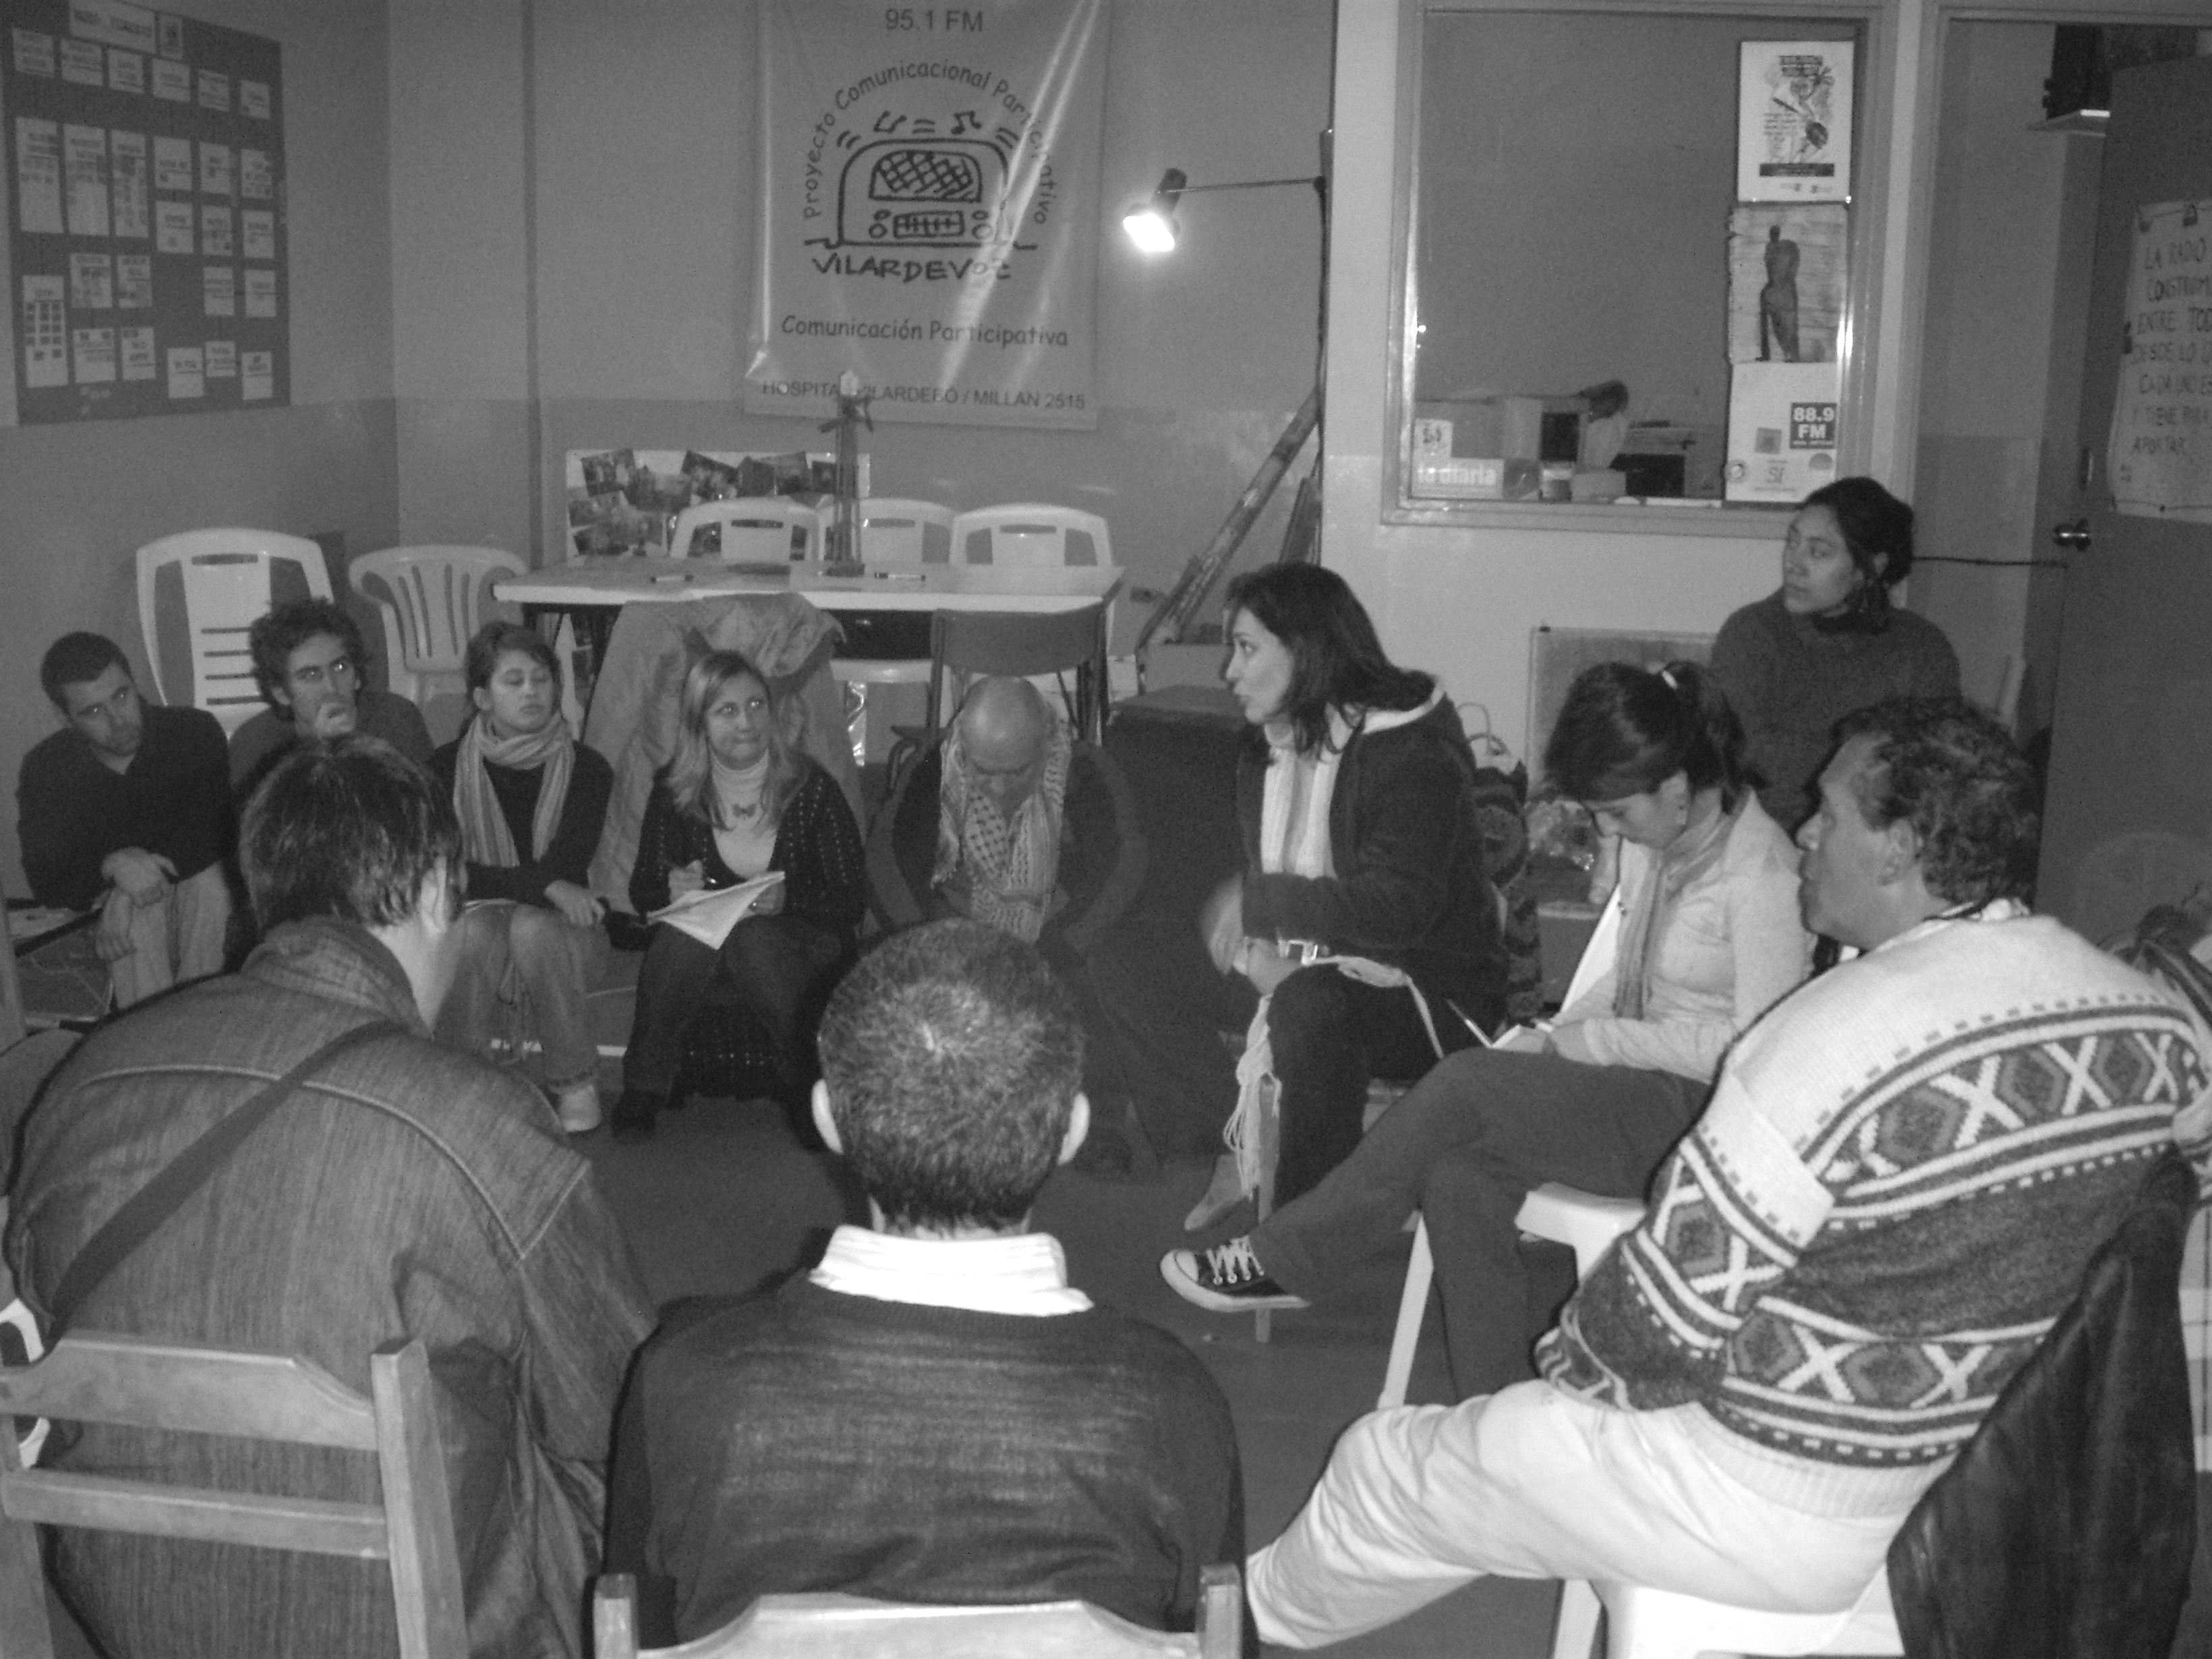
\includegraphics[scale=0.1,keepaspectratio=true]{./Cap/Fotos/Vilarbyn.jpg}
 % Vilarbyn.jpg: 3280x2460 pixel, 96dpi, 86.78x65.09 cm, bb=
 \caption{Taller en radio Vilardevoz, Hospital Vilardebó, Montevideo.}
 \label{Vilarbyn}
\end{figure}

Por otra parte, en el caso de la emisora “Ciudad” de Los Cerrillos (Canelones), se suspendieron los talleres acordados, puesto que la radio estaba en mudanza de local, no pudiéndose establecer nueva instancia de trabajo.\\

Es necesario destacar también que con la radio “El Puente”, La Teja (Montevideo), se realizaron diferentes contactos, pero no se logró realizar ni el taller ni las encuestas.\\

Asimismo, no fue posible relevar información de tres emisoras citadas en la membresía original brindada por AMARC, debido a que las mismas ya no se encontraban funcionando. Este es el caso de “La Gaviota” de Villa García (Montevideo), “Comunitaria” de Soca (Canelones) y “La Quimera” de Atlántida (Canelones).\\

\subsection{Taller nacional}

Se llevó a cabo en el local radial de “El Puente”. Al día siguiente del taller, AMARC tenía Asamblea General. La actividad tuvo alta participación, con al menos un integrante de la mayoría los colectivos. Se trabajó en pequeños grupos, donde cada equipo tenía un documento base, referido a la sistematización de lo relevado en esa área específica. Posteriormente, en plenario general, cada grupo discutió sobre su impresión del documento y relató los aportes que entendía oportunos. Este plenario hizo acuerdo con diversos aportes a ser incluidos en la publicación final. Luego, se realizó una presentación de los datos del Estudio de audiencia. Finalmente se realizó una evaluación del proceso y de los resultados, entregándose el material (papelógrafos y encuestas) a cada colectivo.